% \chapter HARDWARE REQUIREMEN\k'pT}
 %This section  .... table \ref{table:2} \cite{r2}
 \chapter{Hardware Requirements}
\section{All Active Directory VM Hardware Requirements}

\begin{figure}[ht]
    \centering
    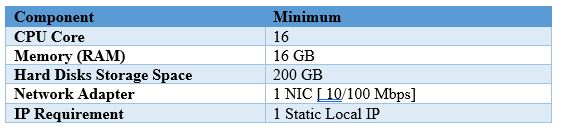
\includegraphics{Chap5/AD-HW.JPG}
    \caption{ADDS HW Requirements}
    \label{fig:ADDS}
\end{figure}
\section{All Mailbox VM Hardware Requirements}
\begin{figure}[ht]
    \centering
    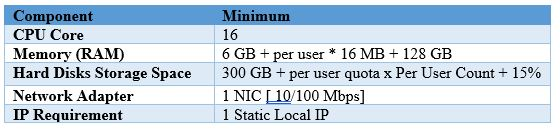
\includegraphics{Chap5/EX-HW.JPG}
    \caption{Mailbox Server HW Requirements}
    \label{fig:MBX}
\end{figure}

\newpage

\section{Reverse Proxy VM Hardware Requirements}
\begin{figure}[ht]
    \centering
    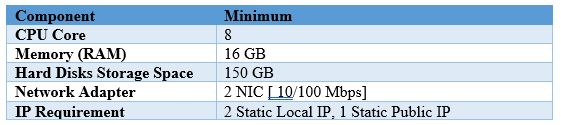
\includegraphics{Chap5/R-Proxy-HW.JPG}
    \caption{Reverse Proxy Server HW Requirements}
    \label{fig:R-Proxy}
\end{figure}
\section{Witness Server VM Hardware Requirements}
\begin{figure}[ht]
    \centering
    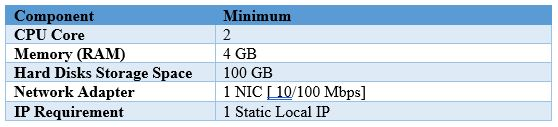
\includegraphics{Chap5/Wit-HW.JPG}
    \caption{Witness Server HW Requirements}
    \label{fig:Witness}
\end{figure}
\section{DNS Server VM Hardware Requirements}
\begin{figure}[ht]
    \centering
    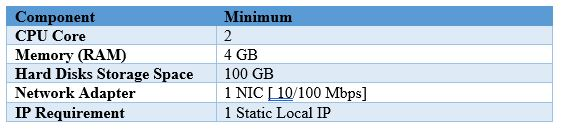
\includegraphics{Chap5/DNS-HW.JPG}
    \caption{DNS Server HW Requirements}
    \label{fig:DNS}
\end{figure}
\newpage

\section{SCCM Server VM Hardware Requirements}
\begin{figure}[ht]
    \centering
    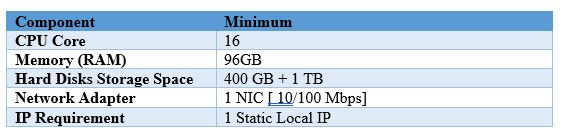
\includegraphics{Chap5/SCCM-HW.JPG}
    \caption{SCCM Server HW Requirements}
    \label{fig:SCCM}
\end{figure}
\section{Functions of Server Resources}
ADDS is the backbone of identity and access management within the enterprise. It authenticates users, enforces security policies, and manages resources across the network. The domain controllers are functioning optimally, with replication across sites verified. Group Policy Objects (GPOs) have been reviewed and updated to reflect recent security enhancements.
DNS ensures reliable name resolution across the network. Internal zones are configured for secure dynamic updates, and forwarders are set to external trusted resolvers. DNS logs indicate healthy query resolution rates, and no significant latency or failures have been observed. Regular scavenging is scheduled to prevent stale records.
The Witness Server plays a critical role in maintaining quorum in cluster environments, particularly for Exchange DAGs and Hyper-V clusters. It is hosted on a separate site to ensure high availability. Recent failover tests confirmed its responsiveness and ability to maintain cluster integrity during node outages. \cite{wiki_2016}
Exchange Server handles enterprise email services. The DAG configuration is stable, with mailbox databases distributed for load balancing. Transport queues are within acceptable thresholds, and backup jobs are completing successfully. Outlook connectivity and OWA access have been tested and verified. No service degradation has been reported.
SCCM is used for endpoint management, software deployment, and patching. The site server is healthy, and distribution points are synchronized. Recent deployments of Windows updates were successful across all client systems. \cite{mondal_automatic_2017}

